\documentclass{article}
\usepackage[utf8]{inputenc}
\usepackage[T1]{fontenc}
\usepackage[francais]{babel}
\usepackage{soul}
\usepackage{ulem}
\usepackage{amsmath}
\usepackage{amsmath}
\usepackage{amssymb}
\usepackage{mathrsfs}
\usepackage{amsthm}
\usepackage{pgfplots}
\usepackage{minted}
\usepackage{listings}
\setlength\parindent{0pt}
\pgfplotsset{}
\newcommand{\norm}[1]{\left\lVert#1\right\rVert^{2}}

\begin{document}
	
	%--------------------------------------------------------------------------------
	% PAGE DE GARDE
	%--------------------------------------------------------------------------------
	\begin{titlepage}
		\centering
		
\includegraphics[width=0.15\textwidth]{ensae.jpg}\par\vspace{1cm}
		{\scshape\LARGE ENSAE ParisTech\par}
		\vspace{1cm}
		{\scshape\Large Projet de Statistiques\par}
		\vspace{1.5cm}
		{\huge\bfseries Introduction à la régression pénalisée et à l'estimateur lasso\par}
		\vspace{2cm}
		{\Large\itshape par Mehdi Abbana Bennani\par
			\Large\itshape et Julien Mattei\par}
		\vspace{2cm}
		supérvisés par\par
		\Large\itshape Pr.~Edwin \textsc{Grappin}\par
		\vfill
		
		% Bottom of the page
		{\large \today\par}
	\end{titlepage}
	
	%---------------------------------------------------------------------------------
	%  FIN PAGE DE GARDE
	%---------------------------------------------------------------------------------
	
	\title{	}
	
	\section{Régression OLS}
	
	\paragraph{Question 1 :}
	\begin{align}
	\intertext{Afin de calculer l'estimateur par moindre carrés, on minimise l'erreur quadratique:}
	\underset{\beta}{min}\norm{ y - X \beta}  \notag
	\intertext{Le gradient de l'erreur quadratique est nul en $\beta^\star$}
	\nabla_{\beta} \norm{ y - X \beta}(\beta^{\star}) = 0 \Longleftrightarrow     &  \nabla_{\beta} (( y - X \beta)^{T} ( y - X \beta)) (\beta^{\star}) = 0
	\notag \\ \Longleftrightarrow &-2X^T y + 2X^T X \beta^\star = 0
	\notag \\ \Longleftrightarrow  &\boxed{\beta^{\star} = (X^{T}X)^{-1}X^{T}y}
	\end{align}
	
	
	Dans la suite on notera $\hat{\beta}$ l'estimateur des moindres carrés.
	
	\paragraph{Question 2:}
	~\par
	
	Le code est disponible en annexe. Nous avons divisé le dataset en un Train Set et en Test Set. La proportion du Train Set est de 90.\%
	Ceci va nous permettre de mesurer l'erreur de prédiction.
	
	La métrique que nous avons choisie pour mesurer cette erreur est la RMSE (Root Mean Square Error), définie par :
	\begin{equation}
	RMSE(\textbf{y}_{\textbf{pred}}, \hat{\textbf{y}})= \frac{1}{|Prediction Set|}\sum_{i=1}^{|Prediction Set|}{(\hat{y}_{i} - y_{i})^2}
	\end{equation}
	
	Nous définissons aussi le $R^2$ la part de variance expliquée par le modèle comme suit:
	\begin{equation}
	R^2 = \frac{\sum_{i=1}^{n}(\hat{y}_{i} - \bar{y})^2}{\sum_{i=1}^{n}(y_{i} - \bar{y})^2}
	\end{equation}
	
	Nous avons obtenu une RMSE de 4.53 sur le test set, et de 3.76 sur le train set. L'écart type estimé sur le Train Set est de l'ordre de 9. On obtient donc une RMSE de l'ordre de 40\% de l'écart type. Il est normal que l'erreur sur le test set soit supérieure à celle mesurée sur le train set, car celui-ci a été utilisé pour estimer le paramètre. Nous avons aussi mesuré le $R^2$ soit la part de variance expliquée sur le train set, nous avons obtenu 96\%, ce qui nous conforte sur la capacité prédictive du modèle. On remarque aussi qu'il n'y a aucun coefficient nul dans le paramètre $\hat{\beta}$ estimé.

	
	\paragraph{Question 3:}
	~\par
	
	On ne peut pas utiliser la régression par moindres carrés si le 
	nombre de variables est supérieur au nombre d'observations
	\begin{proof}
		~\\Soit X est une matrice de dimensions (n,p)
		\vspace{2mm} %5mm vertical space
		\\$X^{T}X$ est une matrice carrée de dimension p
		\vspace{2mm} %5mm vertical space
		\\ On a $rg(X) \leq min(n,p)$ 
		\vspace{2mm} %5mm vertical space
		\\Or $rg(X^{T}X) = rg(X)$
		\vspace{2mm} %5mm vertical space
		\\Donc $rg(X^{T}X) \leq min(n,p)$
		\vspace{2mm} %5mm vertical space
		\\Par hypothèse, le nombre de variables est plus grand que le nombre d'observations, soit $p > n$
		\vspace{2mm} %5mm vertical spac
		\\On en déduit que $rg(X^{T}X) < n $ car $min(n,p) = n$
		\vspace{2mm} %5mm vertical spac
		\\Donc $rg(X^{T}X) < p $ car $n < p$
		\vspace{2mm} %5mm vertical spac
		\\Ainsi $X^{T}X$ est une matrice de taille p dont le rang est strictement inférieur à sa dimension .
		\vspace{2mm} %5mm vertical spac
		\\Donc $X^{T}X$ n'est pas inversible.
		\vspace{2mm} %5mm vertical spac
		\\Conclusion : on ne peut pas utiliser la méthode des moindres carrées dans ce cas.
	\end{proof}
	
	\section{Régression pénalisée : le lasso}
	
	\paragraph{Question 4 :}
	~\par
	\begin{align}
	\intertext{Sous l'hypothèse de p=1, on résout le problème d'optimisation:}
	&\underset{\beta}{min}\frac{1}{2n} \|\textbf{y} - \textbf{X}\beta \|_{2} + \lambda\|\beta\|_{1} \notag
	\intertext{En développant la norme 2 on obtient:}
	&\underset{\beta}{min}\frac{1}{2n}\sum_{i=0}^{n}(y_{i}-x_{i}\beta)^2 + \lambda|\beta| \notag
	\intertext{A partir de l'équation (1), on retrouve la valeur de l'estimateur par moindres carrés $\hat{\beta} = \frac{y}{x}$}
	\intertext{On injecte $\hat{\beta}$ dans le problème d'optimisation:}
	& \underset{\beta}{min} \frac{1}{2n}\sum_{i=0}^{n}x_{i}^{2}\beta^{2} - \frac{1}{n}\sum_{i=0}^{n}x_{i}^{2} \beta \hat{\beta} + \frac{1}{2n}\sum_{i=0}^{n}y_{i}^{2} +
	\lambda|\beta| \notag
	\intertext{On supprime les constantes:}
	& \underset{\beta}{min} \frac{1}{2n}\sum_{i=0}^{n}x_{i}^{2}\beta^{2} - \frac{1}{n}\sum_{i=0}^{n}x_{i}^{2} \beta \hat{\beta} + \lambda|\beta| \notag
	\intertext{On remarque que si $\hat{\beta}<0$ Alors forcément $\beta^{lasso}<0$
		Car les termes en $\beta^2$ et en $|\beta|$ ne dépendent pas du signe de $\beta$, et vu que $\hat{\beta}<0$ alors$-\frac{1}{n}\sum_{i=0}^{n}x_{i}^{2} \hat{\beta}>0$ Donc pour minimiser la quantité, il faut que $\beta^{lasso}<0$  }
	\intertext{De même si $\hat{\beta}>0$ Alors forcément $\beta^{lasso}>0$}
	\intertext{On va traiter les deux cas:}
	\intertext{Si $\hat{\beta}>0$, on résout:}
	& \underset{\beta}{min} \frac{1}{2n}\sum_{i=0}^{n}x_{i}^{2}\beta^{2} - \frac{1}{2n}\sum_{i=0}^{n}x_{i}^{2} \beta \hat{\beta} + \lambda\beta \notag
	\intertext{On obtient:} 
	&\beta^{lasso} = \hat{\beta} - \frac{\lambda}{\sum_{i=0}^{n}\frac{x_{i}^{2}}{2n}} \notag
	\intertext{Or $\beta^{lasso} $ forcément positif, donc}
	&\beta^{lasso} = max(0, \hat{\beta} - \frac{\lambda}{\frac{1}{2n}\sum_{i=0}^{n}x_{i}^{2}}) \notag
	\intertext{Si $\hat{\beta}<0$, à l'aide d'un raisonnement similaire, la seule différence étant $-\lambda$ au lieu de $\lambda$:} 
	&\beta^{lasso} = max(0, \hat{\beta} + \frac{\lambda}{\frac{1}{2n}\sum_{i=0}^{n}x_{i}^{2}}) \notag
	\intertext{On en déduit que:} 
	&\boxed{ \beta^{lasso} = sg(\hat{\beta}) (|\hat{\beta}| - t )_{+}} \text{            avec $t = \frac{\lambda}{\frac{1}{2n}\sum_{i=0}^{n}x_{i}^{2}}$}
	\end{align}
	
	Le seuillage doux permet de régler l'intervalle sur lequel on veut estimer $\beta^{lasso}$. Ainsi, comme le montre la figure \ref{fig:beta_lasso_fenetre} si notre estimateur $\hat{\beta}$ est compris dans l'intervalle $[-t,t]$ il est ramené à 0. On ne retient que les valeurs de $\hat{\beta}$ en dehors de cet intervalle (même principe qu'un filtre).
	\\L'estimateur $\beta^{lasso}$ est nul pour tout les $\hat{\beta}$ dans l'intervalle $[-t,t]$. Donc cela induit une estimation nulle plus souvent que l'estimateur des moindres carrés, celui-ci est nul seulement si $\hat{\beta} = 0$.
	\\t est croissant en $\lambda$, donc en choisissant $\lambda$, nous pouvons modifier la taille du filtre, et donc régler le nombre de coefficients nuls dans notre estimateur, plus $\lambda$ est grand plus le nombre de coefficients nuls est grand.
	
	\begin{figure}
		\centering
		\begin{tikzpicture}
		\begin{axis}[ 
		xlabel=$\hat{\beta}$,
		ylabel={$\hat{\beta} \rightarrow sg(\hat{\beta}) (|\hat{\beta}| - 2 )_{+}$}
		] 
		\addplot {x/ abs(x) *(max(abs(x) - 2, 0))}; 
		\end{axis}
		\end{tikzpicture}
		\caption{$\beta^{lasso}$ en fonction de $\hat{\beta}$ pout $t=2$}
		\label{fig:beta_lasso_fenetre}
	\end{figure}
	
	\paragraph{Question 5:}
	~\par
	Dans la régression pénalisée, en plus du coût de l'erreur de prédiction, on ajoute un coût lié aux valeurs de $\beta$ pour limiter certaines de leurs valeurs possibles. 
	
	Dans le cas du lasso par exemple, toutes les coefficients de l'estimateur par moindres carrées inférieures à t en valeur absolue sont ramenées  zéros, l'intervalle dans lequel $\beta^{lasso}$ peut être non nul est $]-\infty,-t] \cup \left\lbrace0\right\rbrace \cup [t,\infty[$. Dans le cas de la régression Ridge, on pénalise les coefficients trop grands de $\beta^{Ridge}$.
	\vspace{2mm} %5mm vertical space
	\\L'estimateur Lasso est adapté à notre problème car nous allons pouvoir réduire la taille de l'espace des paramètres jusqu'à ce que le nombre de coefficients de beta non nuls soit égal à n (le nombre d'observations), en contrôlant la valeur de $\lambda$. Plus celui-ci est grand, plus le nombre de paramètres nuls sera grand, comme le montre la figure \ref{fig:beta_lasso_fenetre}, car le filtre grandit.
	
	\paragraph{Question 6 :}
	~\par
	
	La pénalisation Ridge a tendance à pénaliser les coefficients dans $\beta$ trop grandes, mais n'a pas tendance à réduire à zéro ces coefficients, contrairement à la pénalisation lasso. Elle est en général utilisée pour limiter le phénomène d'overfitting, en réduisant les valeurs dans $\beta$ en valeur absolue, ce qui diminue la variance des prédictions, réduisant ainsi l'overfitting.
	\\Comme le lasso, la pénalisation $l_{0}$ vise aussi à réduire la taille de l'espace des variables, toutefois le problème d'optimisation associé est NP complet, contrairement à la pénalisation lasso pour laquelle nous avons pu obtenir une expression analytique en dimension 1 et qui peut être approchée en plus grande dimension.

	\paragraph{Question 7 :}
	~\par
	
	Nous avons utilisé le package Glmnet pour calculer l'estimation de $\beta^{lasso}$. La démarche est la même que celle de la question 2. La fonction glmnet cherche par défaut un $\lambda$ optimal, nous avons imposé que la régression lasso soit effectuée pour $\lambda=0.1$, le choix est arbitraire.
	
	On obtient un $R^{2}$ de 0.84 sur le train set, qui laisse penser que le modèle a une bonne capacité prédictive, une RMSE sur le Test set de 3.77, et une RMSE de 2.61 sur le train set. L'écart type sur le Train set est de l'ordre de 10. Donc la qualité de la prédiction est raisonnable en comparaison avec l'écart type de l'échantilllon. 
	
	
	\section{Le choix du paramètre $\lambda$}
	
	\paragraph{Question 8 :}
	~\par
	
	Le paramètre $\lambda$ permet de réduire la taille de l'espace des variables en régleant le nombre de coefficients nuls dans $\beta^{lasso}$. t étant croissant en fonctino de $\lambda$, plus on augmente $\lambda$ plus le filtre est large, plus le nombre de zéros augmente et plus la taille de l'espace des variables est petit.
	
	\paragraph{Question 9 :}
	~\par
	
	Dans la méthode de cross validation, nous divisons le dataset en trois parties: 
	Train Set, Validation Set, et Test Set.
	On entraine le modèle sur le train set puis on estime la qualité de la prédiction sur le validation set pour plusieurs valeurs de $\lambda$, on choisit le lambda le plus performant sur le validation set. Esuite on estime le modèle avec cette valeur de $\lambda$ sur le train set comprenant le train set et le validation set précédents.
	
	\paragraph{Question 10 :}
	~\par
	
	Pour évaluer l'erreur du modèle, nous avons divisé la base de données en Train Set et Test Set, les données du Train Set sont utilisées pour estimer les paramètres, les données du test set sont ensuite utilisés pour évaluer l'erreur d'estimation. La mesure que nous utiliserons est la Root Mean Square Error, définie précédemment. Nous utiliserons aussi le $R^{2}$ défini plus haut.
	
	Pour cette question, nous avons implémenté deux méthodes de cross- validation, l'une automatique à l'aide du package glmnet, et l'autre manuelle en définissant notre propre jeu de paramètres et en divisant la base manuellement.
	
	L'implémentation qui se base sur le package est très simple, il suffit de choisir le nombre de $\lambda$ que l'on veut tester et ensuite effectuer l'estimation.
	
	Pour l'implémentation manuelle, nous avons d'abord choisi un jeu de paramètres $\lambda$ sur une échelle logarithmique. Ensuite nous avons divisé le dataset en Train, Cross-Validation et Test set. Enfin nous avons itéré les estimations de l'erreur sur le Cross-Validation set ensuite nous avons conservé le paramètre avec l'erreur la plus basse.
	
	La méthode automatique s'est révélée plus performante, ce qui est normal car nous n'avons testé que quelques paramètres sur une échelle logarithmique, alors que la méthode automatique teste un jeu de 100 paramètres.	

	Le $R^{2}$ obtenu est identique à celui obtenu sans cross validation, soit 0.83, cela veut dire que notre modèle explique 83\% de la variance de y.

	Comme le montre la figure \ref{nb_zeros_cval}, le nombre de zéros augmente avec lambda, on retrouve l'explication que l'on avait fourni dans la question 6. Lorsque le paramètre $\lambda$ est trop grand, tous les coefficients de $\beta^{lasso}$ sont nuls.
	
	\begin{figure}[ht]
		\centering
		\caption{\label{nb_zeros_cval} Nombre de zéros dans $\beta^{lasso}$ en fonction de $\lambda$, avec $\beta^{lasso} de taile 400$}
		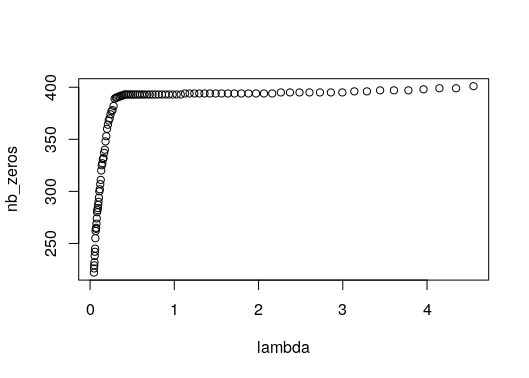
\includegraphics[scale=0.8]{nb_zeros_cval.png}
	\end{figure}

	
	
	
	
	\newpage
	\section{Appendix}


	\inputminted[breaklines, linenos]{R}{main.R}
	
	
	
\end{document}